%This is a LaTeX template for homework assignments
\documentclass{article}

\usepackage[utf8]{inputenc}
\usepackage{amsmath}
\usepackage{amssymb}
\usepackage{graphicx}
\usepackage{enumitem}
\usepackage{multirow}
\usepackage{minted}
\usepackage{multicol}
\usepackage[a4paper, margin=1.2in]{geometry}

\newenvironment{changemargin}[2]{%
\begin{list}{}{%
\setlength{\topsep}{0pt}%
\setlength{\leftmargin}{#1}%
\setlength{\rightmargin}{#2}%
\setlength{\listparindent}{\parindent}%
\setlength{\itemindent}{\parindent}%
\setlength{\parsep}{\parskip}%
}%
\item[]}{\end{list}}

\begin{document}

\thispagestyle{empty}
\begin{center}
\huge
\vspace*{2.0in} EMET8005 
\\\vspace{0.5in} ASSIGNMENT 2
\normalsize
\\\vspace{0.5in} \textsc{By}
\\\vspace{0.1in} \textsc{Zeming Wang}
\\\vspace{0.1in} \textsc{u6114134}
\normalsize
\\\vspace{0.5in} \textsc{Lecturer: Tue Gørgens}
\\\vspace{0.1in} \textsc{Tutor: Luis Uzeda Garcia}
\normalsize
\\\vspace{0.5in} \textsc{Due: May. 15, 2017}
\end{center}

\newpage
\setcounter{page}{1}

\subsection*{A study of the impacts of EITC program on employment}
\begin{enumerate}

\item[(a)]  The sample means and standard deviations (reported in bracket) for age, non-white race, 
years of education, whether working, family income, earnings, and unearned income over the years
1991-1993 for four groups are summarized as below:

    \begin{minted}[fontsize=\footnotesize]{text}
            ------------------------------------------------------------
                                            Number of Children
                                      =0        >0        =1       >=2 
            ------------------------------------------------------------
            Age                     38.27     32.66     33.69     32.00 
            (age)                  [11.16]    [8.50]    [9.82]    [7.46]
                                    
            Non-white                 .50       .64       .56       .69 
            (nonwhite)               [.50]     [.48]     [.50]     [.46]
                                 
            Years of Education       8.53      8.98      8.94      9.01 
            (ed)                    [2.90]    [2.46]    [2.45]    [2.46]
                                 
            Employment                .58       .45       .52       .40  
            (work)                   [.49]     [.50]     [.50]     [.49]
                                 
            Family Income          18,737    12,030    12,706    11,599 
            (finc)                [20,450]  [13,905]  [14,433]  [13,542]
                                 
            Earnings               13,799     7,185     8,711     6,211 
            (earn)                [18,809]  [13,059]  [13,748]  [12,505]
                                 
            Unearned Income         4,938     4,845     3,994     5,387
            (unearn)               [8,433]   [5,691]   [5,435]   [5,785]
                                 
            Earnings if Employed   20,023    12,834    13,828    11,997
            (earn if work)        [19,223]  [13,316]  [13,678]  [12,950]
            ------------------------------------------------------------
    \end{minted}

We can see from the summary table: the mean age of women with no children is much greater than the  
age of women with children; for the groups with more children, the higher the proportion of non-white 
women; the years of education are similar across different groups; the more children they have, 
the less the employment; both family income and earnings have a trend of declining when they 
have more children; while unearned income does not have a clear trend among groups. \\

\item[(b)] To estimate the effect of the EITC program on employment by comparing single women 
with kids and single women without kids, we use the following regression function:
$$ work_i = \gamma + \beta\ anykids_i + u_i $$
where $anykids_i$ is a dummy variable which is $1$ if women $i$ has one or more children
and $0$ otherwise. \\

Run the regression with data in 1994-1996, the output is:

    \begin{minted}[fontsize=\footnotesize]{text}
    ------------------------------------------------------------------------------
                 |               Robust
            work |      Coef.   Std. Err.      t    P>|t|     [95% Conf. Interval]
    -------------+----------------------------------------------------------------
         anykids |  -.0826247   .0125789    -6.57   0.000    -.1072836   -.0579659
           _cons |   .5733862   .0093937    61.04   0.000     .5549715     .591801
    ------------------------------------------------------------------------------    
    \end{minted}

From the regression result, we see that the percentage of employment for women with kids is 
$8\%$ lower than those without kids. \\

This is estimation is prone to bias, because, as the result shown in (a), the characters of 
groups with and without children are very different. This is no way to conclude the decline 
of employment is the causal effect of the EITC program. \\


\item[(c)] Here is a graph for the average annual employment rates for single women with 
children and single women without children from 1991-1996:

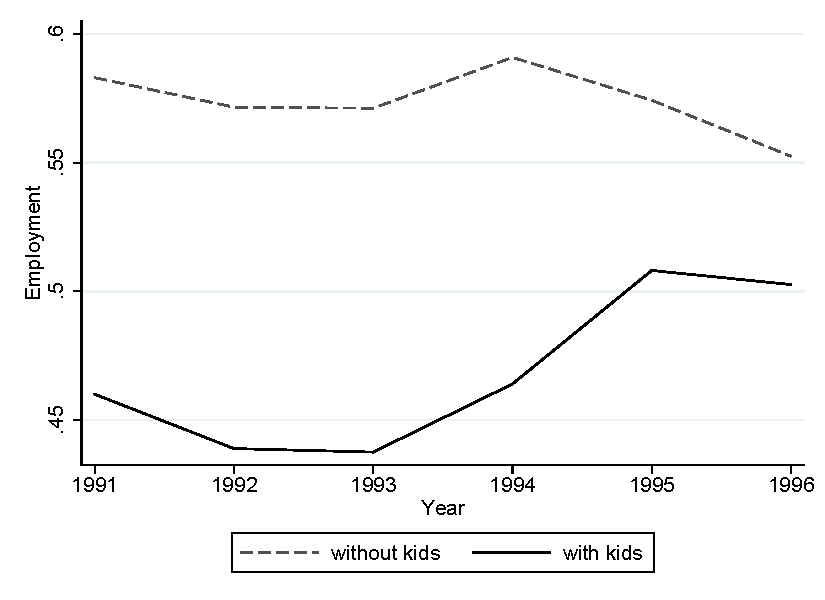
\includegraphics[scale=0.9]{Graph1.pdf}

The trends of employment of the two groups are roughly the same before 1993. From 1993 onward,
when there was a large expansion of the EITC program, the employment of single women with children 
obviously grows faster. \\

So it is reasonable to use single women without children as the control 
group, and use single women with children as the treatment group. Because it looks that they have
a common trend before the treatment comes into effect. \\


\item[(d)] In order to estimate the treatment effect for each year, we use the following regression function:
$$ work_i = \gamma + \beta\ anykids_i + \sum_{t=1991}^{1996}\lambda_t\ year_{ti} + \sum_{t=1991}^{1996}\delta_t\ year_{ti}\times anykids_i + u_i $$

Run the regression with all data from 1991 to 1996, the result is as below:

    \begin{minted}[fontsize=\footnotesize]{text}
    ------------------------------------------------------------------------------
                 |               Robust
            work |      Coef.   Std. Err.      t    P>|t|     [95% Conf. Interval]
    -------------+----------------------------------------------------------------
            year |
           1992  |  -.0114667   .0213317    -0.54   0.591    -.0532797    .0303463
           1993  |  -.0118882   .0215298    -0.55   0.581    -.0540896    .0303132
           1994  |   .0078766   .0215405     0.37   0.715    -.0343457    .0500989
           1995  |  -.0087967   .0220623    -0.40   0.690    -.0520417    .0344484
           1996  |  -.0305527   .0224727    -1.36   0.174    -.0746023     .013497
                 |
         anykids |  -.0498436   .0224787    -2.22   0.027     -.093905   -.0057823
    ------------------------------------------------------------------------------
    \end{minted}
    \begin{minted}[fontsize=\footnotesize]{text}
    Regression Output (Continued)
    ------------------------------------------------------------------------------
    year#anykids |
         1991 1  |  -.0731356   .0298399    -2.45   0.014    -.1316259   -.0146453
         1992 1  |  -.0828017   .0302621    -2.74   0.006    -.1421195    -.023484
         1993 1  |  -.0837539   .0305525    -2.74   0.006     -.143641   -.0238669
         1994 1  |  -.0770339   .0307646    -2.50   0.012    -.1373367    -.016731
         1995 1  |  -.0162656   .0314074    -0.52   0.605    -.0778284    .0452972
         1996 1  |          0  (omitted)
                 |
           _cons |   .5830325   .0148189    39.34   0.000     .5539853    .6120796
    ------------------------------------------------------------------------------
    \end{minted}

Plot the coefficient of the interaction terms $\delta_t$ against years:

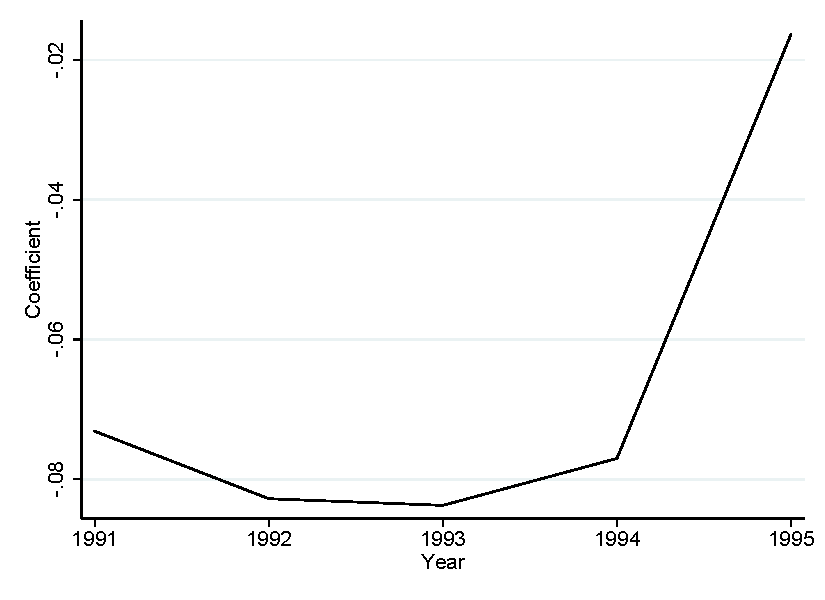
\includegraphics[scale=0.9]{Graph2.pdf}

The difference between the two trends from the treatment group and the control group
shrinks before 1993 but gets enlarged after 1993, and significantly enlarged after 1994. \\

If we hypothesis test the joint significant for the interactions terms for 1991-1993, 
$$ H_0: \delta_{1991}=0,\ \delta_{1992}=0,\ \delta_{1993}=0 $$

we get an $F$-stat of $3.36$ with $p$-value of $0.0179$, which leads us to reject the null
hypothesis with $95\%$ significance level. \\

The dummies $\delta_t$ can be interpreted as the difference of the employment change from 
year to year between the treatment group and the control group (difference in difference). 
We reject the null hypothesis and thus conclude the difference of the two trends are 
significantly different even before 1993. This conclusion differs from our observation in 
part (c) in which the two trends looks rather similar before 1993. \\

\newpage

\item[(e)] Run $t$-test to test the difference between different groups as well as between
different time period, the result is summarized as below (standard errors are reported in parentheses): 

                \begin{minted}[fontsize=\footnotesize]{text}
                    --------------------------------------------------
                                      1991-1993  1994-1996  Difference
                    --------------------------------------------------
                    Treatment Group     .446       .491       -.045
                    (children >0)      (.008)     (.008)      (.011)
                                       
                    Control Group       .575       .573        .002
                    (children =0)      (.009)     (.009)      (.013)
                                       
                    Difference         -.130      -.083       -.047
                                       (.011)     (.013)      (.017)
                    --------------------------------------------------
                \end{minted}

The last bit of the value (difference of difference) is calculated manually by subtracting
the two difference difference values horizontally or vertically, and the standard error 
is calculated by assuming that the sub-samples are independent.
$$ DD = D_1 - D_2,\ SE(DD) = \sqrt{SE^2(D_1) + SE^2(D_2)} $$

\item[(f)] Recalculate the difference in difference estimates between those with one child and 
those with no child. The result is summarized as below (standard errors are reported in parentheses):

                \begin{minted}[fontsize=\footnotesize]{text}
                    --------------------------------------------------
                                      1991-1993  1994-1996  Difference
                    --------------------------------------------------
                    Treatment Group     .524       .554       -.031
                    (children =1)      (.012)     (.013)      (.018)
                                       
                    Control Group       .575       .573        .002
                    (children =0)      (.009)     (.009)      (.013)
                                       
                    Difference         -.052      -.019       -.033
                                       (.015)     (.016)      (.022)
                    --------------------------------------------------
                \end{minted}

And the difference in difference estimates between those with two or more child and 
those with no child. The result is summarized as below:

                \begin{minted}[fontsize=\footnotesize]{text}
                    --------------------------------------------------
                                      1991-1993  1994-1996  Difference
                    --------------------------------------------------
                    Treatment Group     .396       .450       -.053
                    (children >=2)     (.010)     (.011)      (.014)
                                       
                    Control Group       .575       .573        .002
                    (children =0)      (.009)     (.009)      (.013)
                                       
                    Difference         -.179      -.124       -.055
                                       (.013)     (.014)      (.019)
                    --------------------------------------------------
                \end{minted}
                
The last difference in difference values are calculated with the same method as in part (e).\\

The treatment effect for single women with two or more children (-.055) are much larger than those  
with one child (-.033), which is consistent with the fact that those with two or more children 
receives more subsidies from EITC than those with one child. The implication is that the EITC 
program does encourage employment.  

\newpage

\item[(g)] The regression function to estimate the difference-in-difference effect is:
$$ work_i = \gamma + \beta\ anykids_i + \lambda\ post93_i + \delta\ eitc_i + u_i $$
where $eitc_i = anykids_i\times post93_i$ is a new defined dummy variable which is one  
if both $anykids_i$ and $post93_i$ are one, and is zero otherwise.\\

The result of the regression is as following:

\begin{minted}[fontsize=\footnotesize]{text}
--------------------------------------------------------------------------------
               |               Robust
        work   |      Coef.   Std. Err.      t    P>|t|     [95% Conf. Interval]
---------------+----------------------------------------------------------------
     anykids   |  -.1294979    .011648   -11.12   0.000    -.1523296   -.1066662
      post93   |  -.0020735   .0128732    -0.16   0.872    -.0273068    .0231598
anykids#post93 |   .0468731   .0171435     2.73   0.006     .0132695    .0804768
       _cons   |   .5754597   .0088024    65.38   0.000     .5582059    .5927136
--------------------------------------------------------------------------------
\end{minted}

The coefficient of the interaction term ($\approx .047$) and its standard error ($\approx .017$) 
are exactly the same as the values we calculated in part (e). \\

Interpretation of the coefficient: coefficient $\lambda$ and $\beta$ does not have an interpretation
themselves but they helps to unravel the marginal effect of the regressors. 
The marginal effect of having children on employment is:
$$ \frac{\partial\ work}{\partial\ anykids} = \beta + \delta\ post93 $$

The marginal effect of being in treatment years on employment is:
$$ \frac{\partial\ work}{\partial\ post93} = \lambda + \delta\ anykids $$

Coefficient $\delta$ is the difference-in-difference estimate -- how the changes in employment across years 
differ between treatment group and control group. \\


\item[(h)] The regression function  with dummies for each of the years 1991-1996 will be like this:
$$ work_i = \gamma + \beta\ anykids_i + \sum_{t=1991}^{1996}\lambda_t\ year_{ti} + \delta\ eitc_i + u_i $$

Run the regression and the result is as following:

\begin{minted}[fontsize=\footnotesize]{text}
------------------------------------------------------------------------------
             |               Robust
        work |      Coef.   Std. Err.      t    P>|t|     [95% Conf. Interval]
-------------+----------------------------------------------------------------
        year |
       1992  |  -.0170276   .0139552    -1.22   0.222    -.0443817    .0103265
       1993  |  -.0179802   .0141174    -1.27   0.203    -.0456521    .0096918
       1994  |  -.0207379   .0172137    -1.20   0.228     -.054479    .0130032
       1995  |  -.0033267   .0174959    -0.19   0.849     -.037621    .0309675
       1996  |  -.0157367   .0177003    -0.89   0.374    -.0504318    .0189583
             |
     anykids |  -.1295417   .0116483   -11.12   0.000     -.152374   -.1067095
        eitc |   .0469406   .0171451     2.74   0.006     .0133339    .0805474
       _cons |   .5868091   .0117679    49.87   0.000     .5637424    .6098758
------------------------------------------------------------------------------
\end{minted}

Including these year dummies is meant to capture the secular change of employment for each year.
But as we can see, none of the coefficients of the time dummies are statistically significant.
And the treatment effect $\delta$ is almost the same as in part (g) (with only a negligible 
improvement). \\

\item[(i)] In this section we use five different models to estimate the treatment effect.\\

Model 1: The basic model the same as part (h). In the following equations, $\lambda_t$ is used to 
represent all the year dummies for short.
$$ work_i = \gamma + \beta\ anykids_i + \lambda_t + \delta\ eitc_i + u_i $$

Model 2: Control for demographic variables: unearned income, number of children, non-white race, 
age, age squared, years of education, and years of education squared. 
\begin{align*}
work_i = \gamma & + \beta\ anykids_i + \lambda_t + \delta\ eitc_i + \alpha_1\ unearn_i + \alpha_2\ children_i \\ 
                & + \alpha_3\ nonwhite_i  + \alpha_4\ age_i + \alpha_5\ age_i^2 + \alpha_6\ ed_i  + \alpha_7\ ed_i^2 + u_i 
\end{align*}

Model 3: Extend Model 2 by controlling state unemployment rate. The model also allows the effect of  
state unemployment to vary by the presence of children. 
\begin{align*}
work_i = \gamma & + \beta\ anykids_i + \lambda_t + \delta\ eitc_i + \alpha_1\ unearn_i + \alpha_2\ children_i \\
                & + \alpha_3\ nonwhite_i  + \alpha_4\ age_i + \alpha_5\ age_i^2 + \alpha_6\ ed_i  + \alpha_7\ ed_i^2 \\
                & + \alpha_8\ urate_i + \alpha_9\ urate_i\times anykids_i + u_i 
\end{align*}

Model 4: Further extend Model 3 by controlling state-specific effect by including 50 state dummies in the model.
\begin{align*}
work_i = \gamma & + \beta\ anykids_i + \lambda_t + \delta\ eitc_i + \alpha_1\ unearn_i + \alpha_2\ children_i \\
                & + \alpha_3\ nonwhite_i + \alpha_4\ age_i + \alpha_5\ age_i^2 + \alpha_6\ ed_i  + \alpha_7\ ed_i^2 \\
                & + \alpha_8\ urate_i + \alpha_9\ urate_i\times anykids_i \\
                & + \sigma_0\ state0_i + \dots + \sigma_{50}\ state50_i + u_i 
\end{align*}

Model 5: Allowing the treatment effect to vary by those with one or with two or more children. Two new dummy variables 
are defined: $eitc_{1}$ is one for single women with only one child sampled after 1993, and zero otherwise; 
$eitc_{2}$ is one for single women with two or more children sampled after 1993, and zero otherwise.
\begin{align*}
work_i = \gamma & + \beta\ anykids_i + \lambda_t + \delta_1\ eitc_{1i} + \delta_2\ eitc_{2i} + \alpha_1\ unearn_i + \alpha_2\ children_i \\
                & + \alpha_3\ nonwhite_i + \alpha_4\ age_i + \alpha_5\ age_i^2 + \alpha_6\ ed_i  + \alpha_7\ ed_i^2 \\
                & + \alpha_8\ urate_i + \alpha_9\ urate_i\times anykids_i \\
                & + \sigma_0\ state0_i + \dots + \sigma_{50}\ state50_i + u_i 
\end{align*}

The regression results are summarized below. In the actual regression, some variables are scaled 
(unearned income scaled down by a factor of 1000, age squared scaled down by 100, 
and education squared scaled down by 10) in order to make its standard error larger than $0.001$. 
Standard errors are report in parentheses. 

\newpage

        \begin{minted}[fontsize=\footnotesize]{text}
        Table: Regression Result Summary (Model 1-5)
        
        -------------------------------------------------------------------
                                Model    Model    Model    Model    Model        
                 Employment       1        2        3        4        5
        -------------------------------------------------------------------
                       EITC     .047     .058     .049     .038         
              (children >0)    (.017)   (.016)   (.018)   (.018)
                            
                      EITC1                                         .026
              (children =1)                                        (.021)
                                                                                 
                      EITC2                                         .047
             (children >=2)                                        (.019)
                            
                    Anykids    -.130    -.021     .038     .079     .085
              (children >0)    (.012)   (.015)   (.047)   (.047)   (.047)
                            
                   Children             -.052    -.052    -.051    -.054
                                        (.004)   (.004)   (.004)   (.005)
                            
                  Non-White             -.063    -.055    -.069    -.069
                                        (.009)   (.009)   (.010)   (.010)
                                         
            Unearned Income             -.018    -.018    -.017    -.017
              (unearn/1000)             (.001)   (.001)   (.001)   (.001)
                                        
                        Age              .030     .030     .031     .031
                                        (.003)   (.003)   (.003)   (.003)
                                       
                Age Squared             -.038    -.038    -.038    -.038
                (age^2/100)             (.005)   (.005)   (.004)   (.004)
                                         
                  Education             -.004    -.004    -.004    -.004
                                        (.006)   (.006)   (.006)   (.006)
                                         
          Education Squared              .014     .014     .015     .015
                 (ed^2/100)             (.004)   (.004)   (.004)   (.004)
                                        
         State Unemployment                      -.008     .012     .012
                    (urate)                      (.005)   (.008)   (.008)
                                                        
          
           Interaction Term                      -.008    -.013    -.013
          (anykids#c.urate)                      (.006)   (.006)   (.006)
                            
               Year Dummies     Yes      Yes      Yes      Yes      Yes
                            
              State Dummies     No       No       No       Yes      Yes
        -------------------------------------------------------------------
        \end{minted}

In Model 2, we can see non-white single women have 6.3\% lower employment if other things equal.   
And if they have \$1000 more unearned income, their employment falls by 1.8\% holding other things euqal. \\

In Model 3, once the state unemployment rate is controlled, the EITC treatment effect falls from .058 
in Model 2 to .049, which shows that there is a positive bias on the treatment effect when 
state unemployment rate is omitted.\\

The result is not surprising because business cycles affect of the employment of all groups no matter they are subsidized by EITC or not. 
If we plot the average state unemployment rate across years, we will observe a general tendency of the 
unemployment rate to fall.

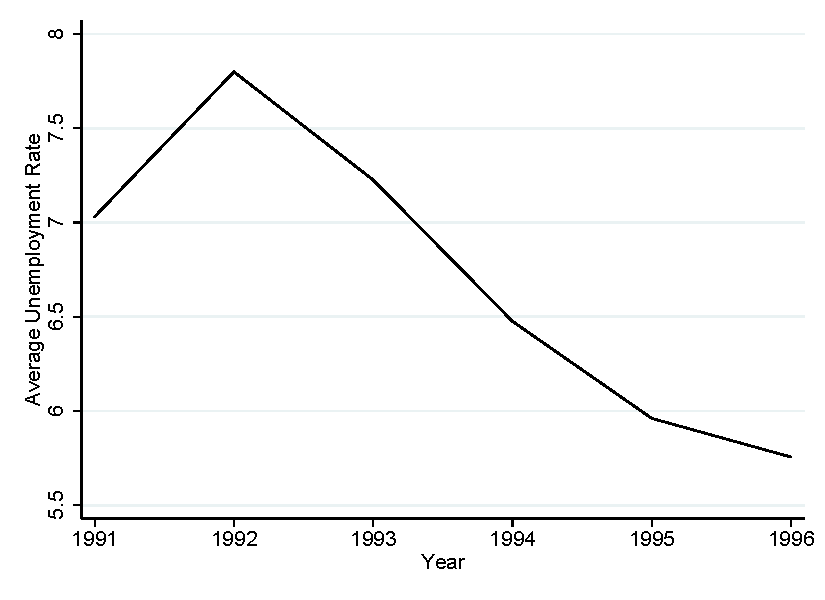
\includegraphics[scale=0.9]{Graph3.pdf}

So some of the employment increase should be attribute to the general fall of unemployment rate but not 
the EITC program. \\

Numerically, 1\% increase in state unemployment rate tends to bring down the employment of single women 
surveyed by 0.8\% (though the number is not statistically significant). And for those with children, 
the downward effect is 0.8\% more severe (suggested by the interaction term, though it is not statistically 
significant either). \\


In Model 4, when we include state-specific dummies, the EITC effect effect further drops down from .049 
in Model 3 to .038 but still remains statistically significant. The change is reasonable because different 
state may have different policies toward low income single women workers (for example some state may provide 
special help to them) so that some of the employment increase could be ascribed to state-specific effect. \\

In Model 5, we estimate the treatment effect separately for those with one child and those with two or more children. 
It is not surprise to find the treatment effect for those with two or more children (.047) is much larger then those 
with only one child (.026), because the EITC program subsidies much more for those with more children. 
The result suggests a positive effect on employment from the expansion of the EITC program. \\

\newpage

\item[(j)] If we try to estimate a fake treatment effect by supposing there was a policy change between 1991 and 1992,  define 1992-1993 as the post-treatment period, the regression function is:
$$ work_i = \gamma + \beta\ anykids_i + \lambda\ post92_i + \delta\ placebo_i + u_i $$
where $placebo_i = anykids_i \times post92_i$, we call it $placebo$ since this is a placebo experiment. \\

Run the regression with data from 1991 to 1993, the result is below:

\begin{minted}[fontsize=\footnotesize]{text}
------------------------------------------------------------------------------
             |               Robust
        work |      Coef.   Std. Err.      t    P>|t|     [95% Conf. Interval]
-------------+----------------------------------------------------------------
     anykids |  -.1229792   .0196214    -6.27   0.000    -.1614428   -.0845157
      post92 |  -.0116737   .0184199    -0.63   0.526     -.047782    .0244346
     placebo |  -.0101282   .0243824    -0.42   0.678    -.0579245    .0376682
       _cons |   .5830325   .0148165    39.35   0.000      .553988     .612077
------------------------------------------------------------------------------
\end{minted}

We can see the placebo treatment effect is very small and not statistically significant.
The placebo experiment thus vindicates our usage of the difference-in-differences methodology 
and makes or result in the above analysis more plausible. 
\end{enumerate}


\newpage

\begin{changemargin}{-0.5in}{-0.5in} 

\subsection*{Appendix: Stata commands and output}

\begin{multicols}{2}

\begin{minted}[fontsize=\tiny]{text}
. use as02.dta                    

. gen anykids = children > 0
. gen post93 = year > 1993
. gen earnw = earn if work 
(6,694 missing values generated)

. //---------------------------- part (a) ----------------------------------
. sum age nonwhite ed work finc earn unearn earnw if !post93 & children == 0

    Variable |        Obs        Mean    Std. Dev.       Min        Max
-------------+---------------------------------------------------------
         age |      3,154    38.26791    11.16455         20         54
    nonwhite |      3,154    .5009512    .5000784          0          1
          ed |      3,154    8.528852    2.898531          0         11
        work |      3,154    .5754597    .4943514          0          1
        finc |      3,154    18736.55    20449.84          0   200190.3
-------------+---------------------------------------------------------
        earn |      3,154    13798.56    18808.73          0   176050.2
      unearn |      3,154    4937.993    8432.572          0   121328.3
       earnw |      1,815    20023.48     19223.1   1.110727   176050.2

. sum age nonwhite ed work finc earn unearn earnw if !post93 & children > 0

    Variable |        Obs        Mean    Std. Dev.       Min        Max
-------------+---------------------------------------------------------
         age |      4,247    32.65811    8.500694         20         54
    nonwhite |      4,247    .6373911    .4808099          0          1
          ed |      4,247    8.983047    2.459027          0         11
        work |      4,247    .4459619    .4971298          0          1
        finc |      4,247    12029.89    13904.87          0   231489.5
-------------+---------------------------------------------------------
        earn |      4,247    7185.022    13058.75          0   162443.6
      unearn |      4,247    4844.867     5691.13          0   102957.9
       earnw |      1,894    12833.91    13315.89   1.178414   108766.8

. sum age nonwhite ed work finc earn unearn earnw if !post93 & children == 1

    Variable |        Obs        Mean    Std. Dev.       Min        Max
-------------+---------------------------------------------------------
         age |      1,654    33.69347    9.822982         20         54
    nonwhite |      1,654    .5592503    .4966271          0          1
          ed |      1,654    8.935308    2.449746          0         11
        work |      1,654    .5235792    .4995948          0          1
        finc |      1,654    12705.66    14433.38          0   158234.9
-------------+---------------------------------------------------------
        earn |      1,654    8711.378    13748.23          0   131557.4
      unearn |      1,654    3994.281    5435.232          0   102957.9
       earnw |        866    13827.82    13678.45   1.178414   96040.75

. sum age nonwhite ed work finc earn unearn earnw if !post93 & children >= 2

    Variable |        Obs        Mean    Std. Dev.       Min        Max
-------------+---------------------------------------------------------
         age |      2,593    31.99769    7.464421         20         54
    nonwhite |      2,593    .6872349     .463709          0          1
          ed |      2,593    9.013498    2.464918          0         11
        work |      2,593     .396452    .4892547          0          1
        finc |      2,593    11598.83     13542.2          0   231489.5
-------------+---------------------------------------------------------
        earn |      2,593    6211.403    12504.98          0   162443.6
      unearn |      2,593    5387.431    5784.552          0   79996.04
       earnw |      1,028    11996.63     12950.2   55.53633   108766.8
 
. //---------------------------- part (b) ----------------------------------
. reg work anykids if post93==1, robust

Linear regression                               Number of obs     =      6,345
                                                F(1, 6343)        =      43.15
                                                Prob > F          =     0.0000
                                                R-squared         =     0.0067
                                                Root MSE          =     .49767

------------------------------------------------------------------------------
             |               Robust
        work |      Coef.   Std. Err.      t    P>|t|     [95% Conf. Interval]
-------------+----------------------------------------------------------------
     anykids |  -.0826247   .0125789    -6.57   0.000    -.1072836   -.0579659
       _cons |   .5733862   .0093937    61.04   0.000     .5549715     .591801
------------------------------------------------------------------------------

. //---------------------------- part (c) ----------------------------------
. // generate average work for women without kids
. egen mwork_nokids = mean (work) if !anykids, by (year) 
(7819 missing values generated)

. // generate average work for women with any kids
. egen mwork_kids = mean (work) if anykids, by (year)
(5927 missing values generated)

. #delimit ;
. graph twoway
> (line mwork_nokids year, sort lcolor(gs5) lpattern(dash))
> (line mwork_kids year, sort lcolor(gs0) lpattern(solid))
> ,
> legend(order(1 "without kids" 2 "with kids"))
> xtitle(year) ytitle(employment)
> ;
. #delimit cr

. //---------------------------- part (d) -------------------------------------
. reg work i.year anykids i.year#anykids, robust

note: 1996.year#1.anykids omitted because of collinearity

Linear regression                               Number of obs     =     13,746
                                                F(11, 13734)      =      17.01
                                                Prob > F          =     0.0000
                                                R-squared         =     0.0134
                                                Root MSE          =     .49669

------------------------------------------------------------------------------
             |               Robust
        work |      Coef.   Std. Err.      t    P>|t|     [95% Conf. Interval]
-------------+----------------------------------------------------------------
        year |
       1992  |  -.0114667   .0213317    -0.54   0.591    -.0532797    .0303463
       1993  |  -.0118882   .0215298    -0.55   0.581    -.0540896    .0303132
       1994  |   .0078766   .0215405     0.37   0.715    -.0343457    .0500989
       1995  |  -.0087967   .0220623    -0.40   0.690    -.0520417    .0344484
       1996  |  -.0305527   .0224727    -1.36   0.174    -.0746023     .013497
             |
     anykids |  -.0498436   .0224787    -2.22   0.027     -.093905   -.0057823
             |
year#anykids |
     1991 1  |  -.0731356   .0298399    -2.45   0.014    -.1316259   -.0146453
     1992 1  |  -.0828017   .0302621    -2.74   0.006    -.1421195    -.023484
     1993 1  |  -.0837539   .0305525    -2.74   0.006     -.143641   -.0238669
     1994 1  |  -.0770339   .0307646    -2.50   0.012    -.1373367    -.016731
     1995 1  |  -.0162656   .0314074    -0.52   0.605    -.0778284    .0452972
     1996 1  |          0  (omitted)
             |
       _cons |   .5830325   .0148189    39.34   0.000     .5539853    .6120796
------------------------------------------------------------------------------

. testparm 1991.year#anykids 1992.year#anykids 1993.year#anykids

 ( 1)  1991b.year#1.anykids = 0
 ( 2)  1992.year#1.anykids = 0
 ( 3)  1993.year#1.anykids = 0

       F(  3, 13734) =    3.36
            Prob > F =    0.0179

. // To plot the coefficient of the interaction terms, create a new dataset with 
. // the coefficient of the interaction terms plot a graph using:
. //     graph twoway line coef year

. //---------------------------- part (e) ----------------------------------
. ttest work if anykids, by(post93) unequal

Two-sample t test with unequal variances
------------------------------------------------------------------------------
   Group |     Obs        Mean    Std. Err.   Std. Dev.   [95% Conf. Interval]
---------+--------------------------------------------------------------------
       0 |   4,247    .4459619    .0076283    .4971298    .4310064    .4609173
       1 |   3,572    .4907615    .0083657    .4999846    .4743595    .5071635
---------+--------------------------------------------------------------------
combined |   7,819    .4664279    .0056421    .4989035    .4553679     .477488
---------+--------------------------------------------------------------------
    diff |           -.0447996    .0113215               -.0669928   -.0226064
------------------------------------------------------------------------------
    diff = mean(0) - mean(1)                                      t =  -3.9570
Ho: diff = 0                     Satterthwaite's degrees of freedom =  7574.24

    Ha: diff < 0                 Ha: diff != 0                 Ha: diff > 0
 Pr(T < t) = 0.0000         Pr(|T| > |t|) = 0.0001          Pr(T > t) = 1.0000

. ttest work if !anykids, by(post93) unequal

Two-sample t test with unequal variances
------------------------------------------------------------------------------
   Group |     Obs        Mean    Std. Err.   Std. Dev.   [95% Conf. Interval]
---------+--------------------------------------------------------------------
       0 |   3,154    .5754597    .0088025    .4943514    .5582006    .5927189
       1 |   2,773    .5733862    .0093939    .4946743    .5549665    .5918059
---------+--------------------------------------------------------------------
combined |   5,927    .5744896    .0064227    .4944619    .5618989    .5870804
---------+--------------------------------------------------------------------
    diff |            .0020735    .0128736               -.0231634    .0273105
------------------------------------------------------------------------------
    diff = mean(0) - mean(1)                                      t =   0.1611
Ho: diff = 0                     Satterthwaite's degrees of freedom =  5827.27

    Ha: diff < 0                 Ha: diff != 0                 Ha: diff > 0
 Pr(T < t) = 0.5640         Pr(|T| > |t|) = 0.8720          Pr(T > t) = 0.4360

. ttest work if !post93, by(anykids) unequal

Two-sample t test with unequal variances
------------------------------------------------------------------------------
   Group |     Obs        Mean    Std. Err.   Std. Dev.   [95% Conf. Interval]
---------+--------------------------------------------------------------------
       0 |   3,154    .5754597    .0088025    .4943514    .5582006    .5927189
       1 |   4,247    .4459619    .0076283    .4971298    .4310064    .4609173
---------+--------------------------------------------------------------------
combined |   7,401    .5011485    .0058124    .5000325    .4897546    .5125424
---------+--------------------------------------------------------------------
    diff |            .1294979     .011648                .1066643    .1523315
------------------------------------------------------------------------------
    diff = mean(0) - mean(1)                                      t =  11.1177
Ho: diff = 0                     Satterthwaite's degrees of freedom =  6813.53

    Ha: diff < 0                 Ha: diff != 0                 Ha: diff > 0
 Pr(T < t) = 1.0000         Pr(|T| > |t|) = 0.0000          Pr(T > t) = 0.0000

. ttest work if post93, by(anykids) unequal

Two-sample t test with unequal variances
------------------------------------------------------------------------------
   Group |     Obs        Mean    Std. Err.   Std. Dev.   [95% Conf. Interval]
---------+--------------------------------------------------------------------
       0 |   2,773    .5733862    .0093939    .4946743    .5549665    .5918059
       1 |   3,572    .4907615    .0083657    .4999846    .4743595    .5071635
---------+--------------------------------------------------------------------
combined |   6,345    .5268716    .0062685    .4993167    .5145833    .5391598
---------+--------------------------------------------------------------------
    diff |            .0826247    .0125789                .0579655     .107284
------------------------------------------------------------------------------
    diff = mean(0) - mean(1)                                      t =   6.5685
Ho: diff = 0                     Satterthwaite's degrees of freedom =  5988.49

    Ha: diff < 0                 Ha: diff != 0                 Ha: diff > 0
 Pr(T < t) = 1.0000         Pr(|T| > |t|) = 0.0000          Pr(T > t) = 0.0000

. //---------------------------- part (f) ----------------------------------
. gen onekid = children==1 if children < 2
  (4,761 missing values generated)

. ttest work if !missing(onekid) &  onekid, by(post93) unequal

Two-sample t test with unequal variances
------------------------------------------------------------------------------
   Group |     Obs        Mean    Std. Err.   Std. Dev.   [95% Conf. Interval]
---------+--------------------------------------------------------------------
       0 |   1,654    .5235792    .0122843    .4995948    .4994848    .5476736
       1 |   1,404    .5541311    .0132703    .4972383    .5280993    .5801628
---------+--------------------------------------------------------------------
combined |   3,058    .5376063    .0090176    .4986653    .5199251    .5552874
---------+--------------------------------------------------------------------
    diff |           -.0305519    .0180833               -.0660088    .0049051
------------------------------------------------------------------------------
    diff = mean(0) - mean(1)                                      t =  -1.6895
Ho: diff = 0                     Satterthwaite's degrees of freedom =  2980.28

    Ha: diff < 0                 Ha: diff != 0                 Ha: diff > 0
 Pr(T < t) = 0.0456         Pr(|T| > |t|) = 0.0912          Pr(T > t) = 0.9544

. ttest work if !missing(onekid) & !onekid, by(post93) unequal

Two-sample t test with unequal variances
------------------------------------------------------------------------------
   Group |     Obs        Mean    Std. Err.   Std. Dev.   [95% Conf. Interval]
---------+--------------------------------------------------------------------
       0 |   3,154    .5754597    .0088025    .4943514    .5582006    .5927189
       1 |   2,773    .5733862    .0093939    .4946743    .5549665    .5918059
---------+--------------------------------------------------------------------
combined |   5,927    .5744896    .0064227    .4944619    .5618989    .5870804
---------+--------------------------------------------------------------------
    diff |            .0020735    .0128736               -.0231634    .0273105
------------------------------------------------------------------------------
    diff = mean(0) - mean(1)                                      t =   0.1611
Ho: diff = 0                     Satterthwaite's degrees of freedom =  5827.27

    Ha: diff < 0                 Ha: diff != 0                 Ha: diff > 0
 Pr(T < t) = 0.5640         Pr(|T| > |t|) = 0.8720          Pr(T > t) = 0.4360

. ttest work if !missing(onekid) & !post93, by(onekid) unequal

Two-sample t test with unequal variances
------------------------------------------------------------------------------
   Group |     Obs        Mean    Std. Err.   Std. Dev.   [95% Conf. Interval]
---------+--------------------------------------------------------------------
       0 |   3,154    .5754597    .0088025    .4943514    .5582006    .5927189
       1 |   1,654    .5235792    .0122843    .4995948    .4994848    .5476736
---------+--------------------------------------------------------------------
combined |   4,808    .5576123    .0071636    .4967214    .5435684    .5716562
---------+--------------------------------------------------------------------
    diff |            .0518805    .0151125                .0222498    .0815113
------------------------------------------------------------------------------
    diff = mean(0) - mean(1)                                      t =   3.4330
Ho: diff = 0                     Satterthwaite's degrees of freedom =  3326.53

    Ha: diff < 0                 Ha: diff != 0                 Ha: diff > 0
 Pr(T < t) = 0.9997         Pr(|T| > |t|) = 0.0006          Pr(T > t) = 0.0003

. ttest work if !missing(onekid) &  post93, by(onekid) unequal

Two-sample t test with unequal variances
------------------------------------------------------------------------------
   Group |     Obs        Mean    Std. Err.   Std. Dev.   [95% Conf. Interval]
---------+--------------------------------------------------------------------
       0 |   2,773    .5733862    .0093939    .4946743    .5549665    .5918059
       1 |   1,404    .5541311    .0132703    .4972383    .5280993    .5801628
---------+--------------------------------------------------------------------
combined |   4,177    .5669141    .0076677    .4955616    .5518813    .5819468
---------+--------------------------------------------------------------------
    diff |            .0192552    .0162587               -.0126251    .0511354
------------------------------------------------------------------------------
    diff = mean(0) - mean(1)                                      t =   1.1843
Ho: diff = 0                     Satterthwaite's degrees of freedom =  2804.91

    Ha: diff < 0                 Ha: diff != 0                 Ha: diff > 0
 Pr(T < t) = 0.8818         Pr(|T| > |t|) = 0.2364          Pr(T > t) = 0.1182


. gen twokids = children>=2 if children !=1
  (3,058 missing values generated)

. ttest work if !missing(twokids) &  twokids, by(post93) unequal

Two-sample t test with unequal variances
------------------------------------------------------------------------------
   Group |     Obs        Mean    Std. Err.   Std. Dev.   [95% Conf. Interval]
---------+--------------------------------------------------------------------
       0 |   2,593     .396452     .009608    .4892547    .3776118    .4152921
       1 |   2,168    .4497232    .0106865    .4975806    .4287665      .47068
---------+--------------------------------------------------------------------
combined |   4,761    .4207099    .0071554    .4937249     .406682    .4347379
---------+--------------------------------------------------------------------
    diff |           -.0532713    .0143706               -.0814446   -.0250979
------------------------------------------------------------------------------
    diff = mean(0) - mean(1)                                      t =  -3.7070
Ho: diff = 0                     Satterthwaite's degrees of freedom =  4582.82

    Ha: diff < 0                 Ha: diff != 0                 Ha: diff > 0
 Pr(T < t) = 0.0001         Pr(|T| > |t|) = 0.0002          Pr(T > t) = 0.9999

. ttest work if !missing(twokids) & !twokids, by(post93) unequal

Two-sample t test with unequal variances
------------------------------------------------------------------------------
   Group |     Obs        Mean    Std. Err.   Std. Dev.   [95% Conf. Interval]
---------+--------------------------------------------------------------------
       0 |   3,154    .5754597    .0088025    .4943514    .5582006    .5927189
       1 |   2,773    .5733862    .0093939    .4946743    .5549665    .5918059
---------+--------------------------------------------------------------------
combined |   5,927    .5744896    .0064227    .4944619    .5618989    .5870804
---------+--------------------------------------------------------------------
    diff |            .0020735    .0128736               -.0231634    .0273105
------------------------------------------------------------------------------
    diff = mean(0) - mean(1)                                      t =   0.1611
Ho: diff = 0                     Satterthwaite's degrees of freedom =  5827.27

    Ha: diff < 0                 Ha: diff != 0                 Ha: diff > 0
 Pr(T < t) = 0.5640         Pr(|T| > |t|) = 0.8720          Pr(T > t) = 0.4360

. ttest work if !missing(twokids) & !post93, by(twokids) unequal

Two-sample t test with unequal variances
------------------------------------------------------------------------------
   Group |     Obs        Mean    Std. Err.   Std. Dev.   [95% Conf. Interval]
---------+--------------------------------------------------------------------
       0 |   3,154    .5754597    .0088025    .4943514    .5582006    .5927189
       1 |   2,593     .396452     .009608    .4892547    .3776118    .4152921
---------+--------------------------------------------------------------------
combined |   5,747    .4946929    .0065957    .5000153    .4817628     .507623
---------+--------------------------------------------------------------------
    diff |            .1790077    .0130306                .1534626    .2045529
------------------------------------------------------------------------------
    diff = mean(0) - mean(1)                                      t =  13.7374
Ho: diff = 0                     Satterthwaite's degrees of freedom =  5553.13

    Ha: diff < 0                 Ha: diff != 0                 Ha: diff > 0
 Pr(T < t) = 1.0000         Pr(|T| > |t|) = 0.0000          Pr(T > t) = 0.0000

. ttest work if !missing(twokids) &  post93, by(twokids) unequal

Two-sample t test with unequal variances
------------------------------------------------------------------------------
   Group |     Obs        Mean    Std. Err.   Std. Dev.   [95% Conf. Interval]
---------+--------------------------------------------------------------------
       0 |   2,773    .5733862    .0093939    .4946743    .5549665    .5918059
       1 |   2,168    .4497232    .0106865    .4975806    .4287665      .47068
---------+--------------------------------------------------------------------
combined |   4,941    .5191257    .0071087    .4996846    .5051895    .5330618
---------+--------------------------------------------------------------------
    diff |             .123663    .0142283                .0957687    .1515572
------------------------------------------------------------------------------
    diff = mean(0) - mean(1)                                      t =   8.6913
Ho: diff = 0                     Satterthwaite's degrees of freedom =  4642.74

    Ha: diff < 0                 Ha: diff != 0                 Ha: diff > 0
 Pr(T < t) = 1.0000         Pr(|T| > |t|) = 0.0000          Pr(T > t) = 0.0000

. //---------------------------- part (g) ----------------------------------
. gen eitc = anykids & post93  
. reg work anykids post93 eitc, robust

Linear regression                               Number of obs     =     13,746
                                                F(3, 13742)       =      58.65
                                                Prob > F          =     0.0000
                                                R-squared         =     0.0126
                                                Root MSE          =     .49674

------------------------------------------------------------------------------
             |               Robust
        work |      Coef.   Std. Err.      t    P>|t|     [95% Conf. Interval]
-------------+----------------------------------------------------------------
     anykids |  -.1294979    .011648   -11.12   0.000    -.1523296   -.1066662
      post93 |  -.0020735   .0128732    -0.16   0.872    -.0273068    .0231598
        eitc |   .0468731   .0171435     2.73   0.006     .0132695    .0804768
       _cons |   .5754597   .0088024    65.38   0.000     .5582059    .5927136
------------------------------------------------------------------------------

. //---------------------------- part (h) ----------------------------------
. reg work i.year anykids eitc, robust 

Linear regression                               Number of obs     =     13,746
                                                F(7, 13738)       =      25.65
                                                Prob > F          =     0.0000
                                                R-squared         =     0.0129
                                                Root MSE          =     .49675

------------------------------------------------------------------------------
             |               Robust
        work |      Coef.   Std. Err.      t    P>|t|     [95% Conf. Interval]
-------------+----------------------------------------------------------------
        year |
       1992  |  -.0170276   .0139552    -1.22   0.222    -.0443817    .0103265
       1993  |  -.0179802   .0141174    -1.27   0.203    -.0456521    .0096918
       1994  |  -.0207379   .0172137    -1.20   0.228     -.054479    .0130032
       1995  |  -.0033267   .0174959    -0.19   0.849     -.037621    .0309675
       1996  |  -.0157367   .0177003    -0.89   0.374    -.0504318    .0189583
             |
     anykids |  -.1295417   .0116483   -11.12   0.000     -.152374   -.1067095
        eitc |   .0469406   .0171451     2.74   0.006     .0133339    .0805474
       _cons |   .5868091   .0117679    49.87   0.000     .5637424    .6098758
------------------------------------------------------------------------------

. //---------------------------- part (i) ----------------------------------
. gen unearn1000 = unearn/1000  
. gen agesq100 = age^2/100 
. gen edsq10 = ed^2/10   
. gen eitc1 = children==1 & post93  
. gen eitc2 = children>=2 & post93

. reg work i.year anykids eitc, robust

Linear regression                               Number of obs     =     13,746
                                                F(7, 13738)       =      25.65
                                                Prob > F          =     0.0000
                                                R-squared         =     0.0129
                                                Root MSE          =     .49675

------------------------------------------------------------------------------
             |               Robust
        work |      Coef.   Std. Err.      t    P>|t|     [95% Conf. Interval]
-------------+----------------------------------------------------------------
        year |
       1992  |  -.0170276   .0139552    -1.22   0.222    -.0443817    .0103265
       1993  |  -.0179802   .0141174    -1.27   0.203    -.0456521    .0096918
       1994  |  -.0207379   .0172137    -1.20   0.228     -.054479    .0130032
       1995  |  -.0033267   .0174959    -0.19   0.849     -.037621    .0309675
       1996  |  -.0157367   .0177003    -0.89   0.374    -.0504318    .0189583
             |
     anykids |  -.1295417   .0116483   -11.12   0.000     -.152374   -.1067095
        eitc |   .0469406   .0171451     2.74   0.006     .0133339    .0805474
       _cons |   .5868091   .0117679    49.87   0.000     .5637424    .6098758
------------------------------------------------------------------------------

. reg work i.year anykids eitc children nonwhite unearn1000 age agesq100 ed edsq10, robust

Linear regression                               Number of obs     =     13,746
                                                F(14, 13731)      =      77.27
                                                Prob > F          =     0.0000
                                                R-squared         =     0.1044
                                                Root MSE          =     .47328

------------------------------------------------------------------------------
             |               Robust
        work |      Coef.   Std. Err.      t    P>|t|     [95% Conf. Interval]
-------------+----------------------------------------------------------------
        year |
       1992  |  -.0149595   .0133492    -1.12   0.262    -.0411258    .0112068
       1993  |  -.0187572   .0134133    -1.40   0.162    -.0450491    .0075347
       1994  |  -.0242385   .0165333    -1.47   0.143     -.056646    .0081691
       1995  |  -.0085387   .0168068    -0.51   0.611    -.0414823     .024405
       1996  |  -.0259888   .0170606    -1.52   0.128    -.0594299    .0074524
             |
     anykids |  -.0209321   .0145209    -1.44   0.149     -.049395    .0075308
        eitc |    .058236   .0163805     3.56   0.000      .026128    .0903441
    children |  -.0518568   .0043387   -11.95   0.000    -.0603613   -.0433523
    nonwhite |   -.062685   .0086142    -7.28   0.000    -.0795699      -.0458
  unearn1000 |  -.0177646   .0011112   -15.99   0.000    -.0199428   -.0155864
         age |   .0301663   .0032812     9.19   0.000     .0237346     .036598
    agesq100 |  -.0377808   .0045024    -8.39   0.000    -.0466062   -.0289554
          ed |  -.0040295   .0059509    -0.68   0.498    -.0156941    .0076351
      edsq10 |   .0142241    .004324     3.29   0.001     .0057485    .0226998
       _cons |    .070401   .0607398     1.16   0.246    -.0486574    .1894593
------------------------------------------------------------------------------

. reg work i.year anykids eitc children nonwhite unearn1000 age agesq100 ed edsq10 
  urate c.urate#anykids, robust

Linear regression                               Number of obs     =     13,746
                                                F(16, 13729)      =      69.30
                                                Prob > F          =     0.0000
                                                R-squared         =     0.1054
                                                Root MSE          =     .47304

---------------------------------------------------------------------------------
                |               Robust
           work |      Coef.   Std. Err.      t    P>|t|     [95% Conf. Interval]
----------------+----------------------------------------------------------------
           year |
          1992  |  -.0053149   .0135492    -0.39   0.695    -.0318732    .0212434
          1993  |  -.0163678   .0134091    -1.22   0.222    -.0426515     .009916
          1994  |  -.0259659   .0171892    -1.51   0.131     -.059659    .0077273
          1995  |  -.0167298   .0177998    -0.94   0.347      -.05162    .0181603
          1996  |  -.0367075   .0180697    -2.03   0.042    -.0721265   -.0012884
                |
        anykids |   .0375987   .0471372     0.80   0.425    -.0547966     .129994
           eitc |   .0485267   .0181173     2.68   0.007     .0130143    .0840391
       children |  -.0521353   .0043406   -12.01   0.000    -.0606435   -.0436271
       nonwhite |  -.0547751   .0089021    -6.15   0.000    -.0722245   -.0373257
     unearn1000 |  -.0176601   .0011094   -15.92   0.000    -.0198347   -.0154855
            age |   .0301347   .0032811     9.18   0.000     .0237033    .0365661
       agesq100 |  -.0377994   .0045031    -8.39   0.000    -.0466261   -.0289727
             ed |  -.0040768   .0059521    -0.68   0.493    -.0157437    .0075902
         edsq10 |   .0137959   .0043271     3.19   0.001     .0053142    .0222776
          urate |  -.0081183   .0047477    -1.71   0.087    -.0174245    .0011879
                |
anykids#c.urate |
             1  |  -.0078118   .0061734    -1.27   0.206    -.0199126     .004289
                |
          _cons |   .1263397   .0689492     1.83   0.067    -.0088102    .2614897
---------------------------------------------------------------------------------

. reg work i.year anykids eitc children nonwhite unearn1000 age agesq100 ed edsq10 
  urate c.urate#anykids i.state, robust

Linear regression                               Number of obs     =     13,746
                                                F(66, 13679)      =      25.88
                                                Prob > F          =     0.0000
                                                R-squared         =     0.1283
                                                Root MSE          =     .46782

---------------------------------------------------------------------------------
                |               Robust
           work |      Coef.   Std. Err.      t    P>|t|     [95% Conf. Interval]
----------------+----------------------------------------------------------------
           year |
          1992  |  -.0174294   .0142025    -1.23   0.220    -.0452684    .0104095
          1993  |  -.0157046   .0133385    -1.18   0.239    -.0418499    .0104408
          1994  |  -.0056221   .0176182    -0.32   0.750    -.0401561     .028912
          1995  |   .0098855   .0193102     0.51   0.609    -.0279651    .0477361
          1996  |  -.0078042   .0199661    -0.39   0.696    -.0469406    .0313321
                |
        anykids |   .0789081    .046958     1.68   0.093     -.013136    .1709522
           eitc |   .0386026   .0179715     2.15   0.032     .0033761    .0738292
       children |  -.0507788   .0043199   -11.75   0.000    -.0592463   -.0423113
       nonwhite |  -.0690147    .009789    -7.05   0.000    -.0882024    -.049827
     unearn1000 |  -.0170273    .001089   -15.64   0.000    -.0191619   -.0148927
            age |   .0306563   .0032553     9.42   0.000     .0242754    .0370371
       agesq100 |  -.0379952   .0044676    -8.50   0.000    -.0467523   -.0292381
             ed |  -.0043077   .0059213    -0.73   0.467    -.0159143    .0072988
         edsq10 |   .0153572   .0043143     3.56   0.000     .0069007    .0238138
          urate |   .0122759   .0081588     1.50   0.132    -.0037164    .0282682
                |
anykids#c.urate |
             1  |  -.0132905   .0061526    -2.16   0.031    -.0253505   -.0012306
                |
          state |
            12  |   .1124645   .0767773     1.46   0.143    -.0380295    .2629586
            13  |   .1702433   .0851066     2.00   0.045     .0034227     .337064
                :
                :   (more output omitted)
                |
          _cons |  -.1748605   .0988185    -1.77   0.077    -.3685584    .0188373
---------------------------------------------------------------------------------

. reg work i.year anykids eitc1 eitc2 children nonwhite unearn1000 age agesq100 ed 
  edsq10 urate c.urate#anykids i.state, robust

Linear regression                               Number of obs     =     13,746
                                                F(67, 13678)      =      25.53
                                                Prob > F          =     0.0000
                                                R-squared         =     0.1284
                                                Root MSE          =     .46781

---------------------------------------------------------------------------------
                |               Robust
           work |      Coef.   Std. Err.      t    P>|t|     [95% Conf. Interval]
----------------+----------------------------------------------------------------
           year |
          1992  |   -.017458   .0142024    -1.23   0.219    -.0452967    .0103807
          1993  |  -.0157295   .0133384    -1.18   0.238    -.0418745    .0104156
          1994  |  -.0056799   .0176206    -0.32   0.747    -.0402187    .0288588
          1995  |   .0099802   .0193093     0.52   0.605    -.0278687    .0478291
          1996  |  -.0077372   .0199635    -0.39   0.698    -.0468683     .031394
                |
        anykids |   .0847147   .0472016     1.79   0.073    -.0078069    .1772363
          eitc1 |   .0255503   .0212377     1.20   0.229    -.0160784    .0671791
          eitc2 |   .0471497   .0192826     2.45   0.014     .0093531    .0849463
       children |  -.0536716   .0048531   -11.06   0.000    -.0631843   -.0441588
       nonwhite |  -.0689486   .0097898    -7.04   0.000     -.088138   -.0497591
     unearn1000 |  -.0170281   .0010892   -15.63   0.000    -.0191631   -.0148931
            age |   .0306172   .0032552     9.41   0.000     .0242365    .0369979
       agesq100 |  -.0379226   .0044679    -8.49   0.000    -.0466802    -.029165
             ed |    -.00441   .0059225    -0.74   0.457     -.016019     .007199
         edsq10 |   .0154401   .0043158     3.58   0.000     .0069806    .0238996
          urate |   .0123086    .008158     1.51   0.131    -.0036821    .0282994
                |
anykids#c.urate |
             1  |  -.0132405   .0061522    -2.15   0.031    -.0252996   -.0011814
                |
          state |
            12  |   .1129185   .0767439     1.47   0.141    -.0375101    .2633471
            13  |   .1692609   .0849943     1.99   0.046     .0026604    .3358614
                :
                :   (more output omitted)
                |
          _cons |  -.1741941   .0988255    -1.76   0.078    -.3679056    .0195174
---------------------------------------------------------------------------------

. //---------------------------- part (j) ----------------------------------

. gen placebo = post92 & anykids
. reg work anykids post92 placebo if year<=1993, robust

Linear regression                               Number of obs     =      7,401
                                                F(3, 7397)        =      42.00
                                                Prob > F          =     0.0000
                                                R-squared         =     0.0167
                                                Root MSE          =     .49594

------------------------------------------------------------------------------
             |               Robust
        work |      Coef.   Std. Err.      t    P>|t|     [95% Conf. Interval]
-------------+----------------------------------------------------------------
     anykids |  -.1229792   .0196214    -6.27   0.000    -.1614428   -.0845157
      post92 |  -.0116737   .0184199    -0.63   0.526     -.047782    .0244346
     placebo |  -.0101282   .0243824    -0.42   0.678    -.0579245    .0376682
       _cons |   .5830325   .0148165    39.35   0.000      .553988     .612077
------------------------------------------------------------------------------
. 
\end{minted}

\end{multicols}
\end{changemargin}


\end{document}